\section{Technical fundamentals}

This section will explain the technical fundamentals which are necessary to understand the full bachelor thesis.

\subsection{The Scapy library}
\label{sec:scapy}

%UDS stack
\begin{wrapfigure}{r}{0.15\textwidth}
    %
\includegraphics[width=0.1\textwidth]{scapy_logo}
    \raisebox{0pt}[\dimexpr\height-1.5\baselineskip\relax]{
\includegraphics[width=0.15\textwidth]{scapy_logo}}
    %\label{fig:scapy-logo}
\end{wrapfigure}

Scapy is a powerful interactive packet manipulation program. It is able to forge or decode packets of a wide number of protocols, send them on the wire, capture them, match requests and replies, and much more \cite{scapy}.

It is used through a text-based user interface. This has the advantage of being very lightweight, and also work via a ssh connection out-of-the-box. While being mainly a program, it can also be used as a library by importing the necessary classes and interfaces into the own Python program. Scapy supports Python 3 and additionally Python 2, even though its support has ended on 1st of January 2020. The following quote from a maintainer explains the reason behind that \cite{scapy-py2}:

\begin{displayquote}
    Scapy is a tool that can be used in a very large number of situations. Often, you don't get to choose the Python interpreter you have when you run Scapy. So, [...] we need to keep supporting Python 2.7 as long as we can.
\end{displayquote}

Understanding Scapy will be important for the later implementation in this work, since the UDS Scanner to be modified is built within Scapy.

One of the core classes in Scapy is the \textbf{Packet} class. All definitions of network packet layers, such as Ethernet, IP, TCP, CAN, UDS and so on, are defined in a class inheriting from that class.

The well-known and simple UDP protocol \cite{rfc768} serves as an illustrative example. It will be shown how the UDP header, shown in \autoref{fig:uds_header}, is translated to such a Scapy class.

%UDP header
\begin{figure}[h]
    \centering
    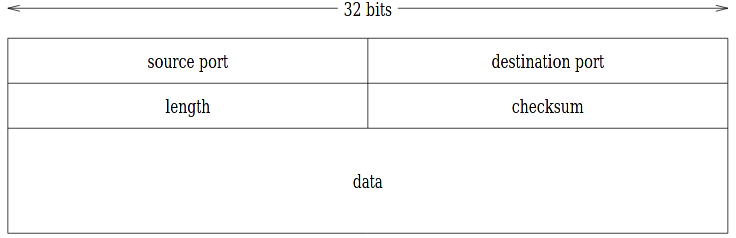
\includegraphics[width=0.7\textwidth]{udp_header}
    \caption{UDP header format \cite{udp_header}}
    \label{fig:uds_header}
\end{figure}

The UDP header format contains four fields and the data field. These four fields are translated literally into the Scapy class \textbf{UDP}. The data field is not part of it because Scapy uses an explicit operator to append data to the header information. This is shown later.

The following code snippet shows the mentioned class in the Scapy library.

\begin{samepage}
\begin{minted}{python}
class UDP(Packet):
   fields_desc = [ShortEnumField('sport', 53, UDP_SERVICES),
                  ShortEnumField('dport', 53, UDP_SERVICES),
                  ShortField('len', None),
                  XShortField('chksum', None)]
\end{minted}
\end{samepage}

As in common programmer language, \textbf{short} specifies 16 bits. Since the UDP header only contains 16 bits fields, the Scapy definition only includes \textbf{short} fields. The first parameter of a field is always the name of this field. \textbf{sport} stands for source port, and \textbf{dport} for destination port.
The next parameter sets the default value for this field. This is defined by the Scapy programmers in all conscience and not by the official UDP standard. \textbf{53} specifies the DNS protocol.
\textbf{EnumField}s also contain a third argument, a simple dictionary mapping from machine-readable values to human-readable texts. For example, part of the \textbf{UDP\_SERVICES} dictionary is: \mintinline{python}{{53: 'domain', 80: 'www_http'}}.
The difference between ShortField and XShortField is only the representation. The value of the XShortField will be displayed as a hex value and the ShortField as a decimal value.

The following snippet shows some examples of how to instantiate an object of the UDP class and also demonstrates how to append data to the headers with the “/” operator.

\begin{samepage}
\begin{minted}{python}
packet = UDP(dport=80) # is equivalent to:
packet = UDP(dport='www_http')

# Append 0x00 as data
packet = UDP(dport=80) / Raw(b'\x00')
\end{minted}
\end{samepage}

Now it shall be explained, how to actually send a packet and receive a response. For this, a socket is required. Scapy provides many kinds of sockets for different use cases. For example the \textbf{L2Socket} and the \textbf{L3PacketSocket}. The difference between them is that L2Socket expects a packet object containing all information starting from Ethernet (Layer 2), while L3PacketSocket expected a packet object only containing all information starting from IP (layer 3). The following code snippet uses the L2Socket for full coverage of the whole packet stack and explains how sending and receiving of a packet works (Note: Root privileges might be necessary for this to work):

\begin{samepage}
\begin{minted}{python}
# import necessary classes
from scapy.arch.linux import L2Socket
# Create a layer 2 socket specifing the interface name
socket = L2Socket('eth0')
# Create a packet covering layer 2 to 7, targeting the Google server
# This packet starts a TCP handshake, thus the SYN flag is exclusively set
# Set destination port to HTTP and a high source port
packet = Ether() / IP(dst='142.250.185.163') / TCP(flags='S', dport=80, sport=60123)
# sr1 stands for: send receive one
# it sends the given packet and returns the response
response = socket.sr1(packet)
# This displays the response in a human-friendly form
response.show()
\end{minted}
\end{samepage}

The .show() command gives the following output. It has been slightly edited to be more compact and some information has been replaced by placeholders for privacy reasons.

\begin{samepage}
\begin{minted}{text}
###[ Ethernet ]### 
  dst       = 12:34:45:67:89:ab
  src       = 2c:3a:fd:af:64:e0
  type      = IPv4
###[ IP ]### 
     version   = 4
     src       = 142.250.185.163
     dst       = 123.123.123.123
###[ TCP ]### 
        sport     = www_http
        dport     = 60123
        flags     = SA
\end{minted}
\end{samepage}

The SYN and ACK flags are now set as expected for the TCP handshake. Furthermore, the sport of the request is the dport of the response.


\subsection{The CAN bus}

All communication performed and recorded in this paper with an ECU is done via the Control Area Network bus.

\subsubsection{Basic information}

 Its specification is released in the ISO 11898. One packet on this bus can only transmit 8 bytes of payload.
 Each CAN packet has an identifier which a length of either 11 or 29-bits, the former being more common. An identifier does not necessarily have to designate a physical device; it can also specify one of several modules in that device.
 The maximum data rate is 1 Mbit/sec with a network length below 40 m. The higher the length, the lower the possible data rate, as can be seen in \autoref{tab:can-speed}.

\begin{table}[h]
    \centering
    \begin{tabular}{|c|c|c|}
    \hline
    \textbf{Bus Length (m)} & \textbf{Signaling Rate (Mbps)}\\
    \hline
    40 & 1 \\
    \hline
    100 & 0.5 \\
    \hline
    200 & 0.25 \\
    \hline
    500 & 0.10 \\
    \hline
    1000 & 0.05 \\
    \hline
\end{tabular}
\caption{Suggested Cable Length vs Signaling Rate \cite{slla270}.}
\label{tab:can-speed}
\end{table}

\subsubsection{Advantages}

This bus is robust because it is half-duplex, but still using two wires for the communication with differential signals. This means that if one wire is driven high, the other one is driven low. Thus, the receiver can reliably detect interferences by comparing these signals.

Moreover, CAN busses are using the bus network topology. This results in a smaller number of wires compared to star topologies, resulting in lower weight, which is an important factor for manufacturers (see \autoref{fig:with-without-can}).

%with-without-can
\begin{figure}[h]
    \centering
    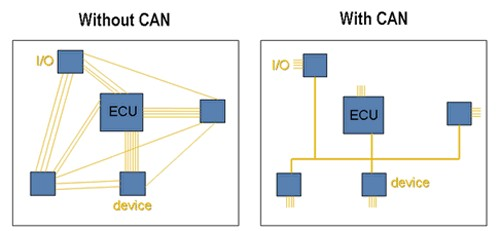
\includegraphics[width=0.7\textwidth]{with-without-can}
    \caption{CAN effect on decreasing the wire quantity \cite{Sharma2016}.}
    \label{fig:with-without-can}
\end{figure}

Last but not least, an important feature for the automotive application domain is the priority support. The lower the identifier, the higher the priority. Hence, if ECU1 and ECU2 transmit a CAN packet at exactly the same time, the packet with the lower identifier wins, the other one is discarded and will be retransmitted. This is called the Carrier Sense Multiple Access with Collision Detection (CSMA/CD) protocol \cite{Sharma2016}.

\subsubsection{Security vulnerabilities}

Thinking this one step further, CAN is vulnerable to denial of service attacks. This attack can be performed by flooding the CAN bus with zero-identifier messages resulting in drops of legitimate packets \cite{Buttigieg2017}.

Furthermore, Buttigieg et al. \cite{Buttigieg2017} describe three more security issues of the CAN bus protocol in their paper {Security Issues in Controller Area Networks in Automobiles}.
First, CAN packets do not contain any authentication information. An ECU receiving a message is not able to distinguish between a message from a legitimate ECU and a malicious one \cite{Buttigieg2017}. So, for example, if an ECUs state is changed to a higher privileged state, all devices, including malicious ones, will have access to its newly unlocked services. Countermeasures exist in the form of performing authentication, but there is no satisfying solution yet, which fulfills cost-effectiveness, backward compatibility, support for vehicle repair and maintenance, sufficient implementation details, and acceptable overhead \cite{Bozdal2020}.
Also, originally, CAN bus networks lacked network segmentation, since each message is broadcasted and received by each node of the network \cite{Buttigieg2017}. Nowadays, car networks of higher-class cars like Audi and BMW are usually divided into less and more critical segments by so-called Gateway ECUs \cite{Bozdal2020}. Despite the increase in the level of security, this makes it more difficult to maintain the system, which is associated with increased costs \cite{Bozdal2020}.
The final security vulnerability is the lack of data encryption \cite{Buttigieg2017}. Lightweight encryption systems could be implemented, but are limited by the short length of the data field (8 bytes) and the limited computing power of the ECUs \cite{Bozdal2020}.

Since all countermeasures described in the previous paragraph are limited, Intrusion Detection Systems (IDS) are emerging, with the advantages of not having to change the current CAN controller and not increasing bus traffic \cite{Bozdal2020}. Such a system has been implemented in the context of the PetS3 project \cite{spahn2018}.

\subsubsection{How to work with the CAN bus}

CAN interfaces are quite expensive, to communicate with ECUs paper the PCAN-USB from PEAK System was used in this work which costs by time of writing 180€. Instead, a virtual CAN interface can be used for simulations or simple tests. This is supported natively by Linux without additional actions.
To create a virtual CAN interface, only one command in a Linux shell is required:
\begin{samepage}
\begin{minted}{text}
sudo ip link add vcan0 type vcan
\end{minted}
\end{samepage}

The most common tool set to work with the CAN bus are the can-utils \cite{can-utils}, which can be usually installed with the package manager of the distributions. For example, the following command displays all messages of the CAN bus on interface \emph{vcan0}:
\begin{samepage}
\begin{minted}{text}
candump vcan0
\end{minted}
\end{samepage}

Another important task is to send a packet, which can be done with:
\begin{samepage}
\begin{minted}{text}
cansend vcan0 123#01.02
\end{minted}
\end{samepage}

This sends a CAN packet with the identifier 0x123 and the payload \emph{01 02}.

Alternatively, Scapy can be used. There are two implementations of CAN sockets, namely a native one, which uses the native Linux kernel module, and a software-based one, which uses the Python-CAN package.  The native implementation is only usable for Linux but the preferred one because it uses the socket interface of Linux and brings all its advantages, such as waiting for answers asynchronously while the own process doesn't require any CPU time. Python-CAN has the advantage of also working on Windows and macOS.

An equivalent Scapy script which accomplishes the same as the just described \mintinline{text}{cansend} command, is:

\begin{samepage}
\begin{minted}{python}
from scapy.contrib.cansocket_native import CANSocket
from scapy.layers.can import CAN
socket = CANSocket("vcan0")
socket.send(CAN(identifier=0x123, data=b"\x01\x02"))
\end{minted}
\end{samepage}

\subsection{The ISO-TP transport protocol for CAN}

CAN packets have a payload size of 8 bytes. This is sufficient for most UDS requests, but not for many UDS responses. Thus, ISO-TP is used as the transport protocol on the CAN bus for UDS communication.

\subsubsection{Basic information}

It is defined in ISO 15765-2 and increases the payload size from 8 bytes to 4095 bytes per message. At least one byte of each CAN packet is then transport protocol information, indicating whether this packet is a single frame or if it only contains a fragment of the actual payload.

\subsubsection{How to work with the ISO-TP protocol}

The can-utils tools also contain applications to handle ISO-TP communication. Since this is never used in this work, but the Scapy implementation is, only the Scapy implementation is explained.

As for the CAN implementation, there are two ISO-TP socket implementations in Scapy. A software and a native implementation. Until including Linux kernel 5.9, the corresponding ISO-TP module for Linux had to be installed separately \cite{isotp-module}. Since Linux kernel 5.10, it is part of the Linux mainline kernel \cite{isotp-commit}. Both implementations handle the ISO-TP metadata themselves, i.e.  fragmentation, defragmentation, etc.

An ISO-TP socket contains a source and destination identifier. They offer the same functionality as the ports for TCP or UDP. The source identifier is the identifier the outgoing CAN packets will contain. The destination identifier is the identifier expected for incoming packets.

The usage of the native implementation is illustrated in the following code snippet:

\begin{samepage}
\begin{minted}{python}
from scapy.contrib.isotp import ISOTPNativeSocket
socket = ISOTPNativeSocket('vcan0', sid=0x123, did=0x456)
packet = Raw(b'\x01\x02')
socket.send(packet)
\end{minted}
\end{samepage}

\subsection{The UDS protocol}

\subsubsection{Basic information}

UDS stands for \emph{Unified diagnostic services} and is an application protocol defined in ISO 14229 \cite{iso14229}. This protocol defines the structures of request and response packets for diagnostic purposes sent over an arbitrary data link.

%UDS stack
\begin{figure}[h]
    \centering
    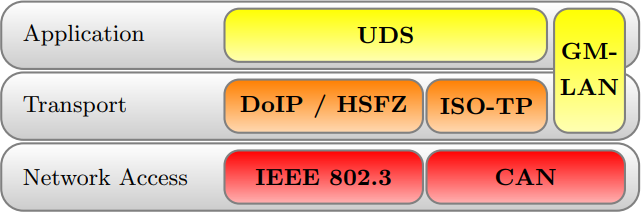
\includegraphics[width=0.7\textwidth]{uds-stack}
    \caption{The most common protocol stack for UDS \cite{Weiss2020}.}
    \label{fig:uds-stack}
\end{figure}

As shown in \autoref{fig:uds-stack}, the most common data links for the UDS protocol are the Ethernet and the CAN bus. Others can and are used as well, explicitly stated in the UDS standard are FlexRay, K-Line and LIN.

\subsubsection{Services}

The UDS protocol defines various services with different purposes. For example, the DiagnosticSessionControl service is used to enable different diagnostic states in the ECU. Its identifier is the number 0x10. All packets requesting this service specify this value as the first byte. The identifiers in the responses are defined as 0x40 added to the request identifier. Thus, for the DiagnosticSessionControl the positive response identifier is 0x10 + 0x40 = 0x50. A negative response always has the identifier 0x7f. This service is able to change the state of the ECU. Although the ReadDataByIdentifier service is not able to change the state, it is still very important. Data records in an ECU are stored with an identifier as the key. This service allows to read these values from an external device. Since there can be data stored, which is not meant to be read by everybody, there is another service called SecurityAccess, which allows to unlock these information for external devices. This mechanism is used for other services as well. The SecurityAccess service uses the challenge–response authentication in which an algorithm is the secret. It follows the following sequence \cite{iso14229}:

\begin{samepage}
\begin{enumerate}
  \item client requests the “Seed”,
  \item server sends the “Seed”,
  \item client sends the “Key” (appropriate for the Seed received),
  \item server responds that the “Key” was valid and that it will unlock itself.
\end{enumerate}
\end{samepage}

Now the implementation of UDS in Scapy is described.

\begin{samepage}
\begin{minted}{python}
class UDS(ISOTP):
    services = {
         0x10: 'DiagnosticSessionControl',
         # [...]
         0x22: 'ReadDataByIdentifier',
         # [...]
         0x7f: 'NegativeResponse'})
    fields_desc = [
        XByteEnumField('service', 0, services)
    ]
\end{minted}
\end{samepage}

%TODO: Why inherting from ISOTP

The UDS class contains only the service field. Even though the whole UDS protocol is in the application layer, the Scapy implementation starts a new class whenever the subsequent fields depend on one field of the current layer. This is the case here, since the next fields depend on the value of the service field. The service specific fields are defined in their own classes, for example:

\begin{samepage}
\begin{minted}{python}
class UDS_DSC(Packet):
    diagnosticSessionTypes = { ... }
    fields_desc = [
        ByteEnumField('diagnosticSessionType', 0,  diagnosticSessionTypes)
    ]
\end{minted}
\end{samepage}

A UDS packet enabling the extendedDiagnosticSession would be created with:

\begin{samepage}
\begin{minted}{python}
packet = UDS() / UDS_DSC(diagnosticSessionType='extendedDiagnosticSession')
\end{minted}
\end{samepage}

UDS not only allows to read data, but also to write. Which makes it especially critical for security. For example the firmware of an ECU can be updated through this protocol. This usually requires higher privileges, which can be gained through the previously mentioned SecurityAccess service.


\subsection{The UDS Scanner}

The UDS Scanner was implemented in Scapy for the PetS3 project.

\subsubsection{Purpose}

\begin{figure}[h]
    \centering
    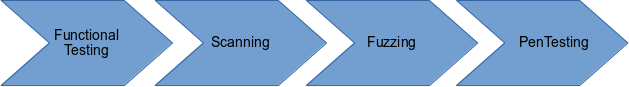
\includegraphics[width=0.8\textwidth]{automotive-security-testing-process}
    \caption{The Automotive Security Testing process.}
    \label{fig:automotive-security-testing-process}
\end{figure}

As \autoref{fig:automotive-security-testing-process} shows, the security testing process in the automotive domain consists of a scanning step \cite{Bayer2015}. This step aims detect which services of a protocol are implemented and what information can be retrieved there. The UDS Scanner fulfills these tasks. It can also be used for fuzzing and functional testing, even though scanning is its main use-case. The retrieved information assists for the manual PenTesting, the last step in this process.

\subsubsection{Enumerators}

% TODO: Add that it was still work in progress while doing this work
% and thus, that problems occured and had to be fixed.
% Out of scope of this work.

It executes so-called Enumerators which are service-specific and create all possible packets for a service.
For example, the enumerator for the DiagnosticSessionControl (DSC) service is called UDS\_DSCEnumerator. The most important member of the enumerator classes is the \mintinline{python}{_get_initial_requests} method. The return value is an iterable object which contains all requests for this service. DSC has an eight bit identifier, leading to a maximum of 2\textsuperscript{8} packets for this service. Each enumerator will be executed for each found state of the ECU. So, if an enumerator already ran, and afterwards a new state is found, this enumerator will run again within the same scan with the new-found state.

For a better understanding, the UDS\_DSCEnumerator implementation will be described exemplary.

\begin{samepage}
\begin{minted}{python}
class UDS_DSCEnumerator(UDS_Enumerator, StateGenerator):
    def _get_initial_requests(self, **kwargs):
        session_range = kwargs.pop('session_range', range(2, 0x100))
        return UDS() / UDS_DSC(diagnosticSessionType=session_range)
\end{minted}
\end{samepage}

The method can be given keyword parameters. The only one used here is \mintinline{python}{session_range}. If none is given, which is usually the case, it defaults to the range from 0x02 to 0xff. So, this enumerator creates 254 packets for each state. This service is a StateGenerator, which means its requests can change the state of the ECU. This is detected by the UDS Scanner and the new state will be scanned as well.

The enumerators can output their results as a text-table. For example:

\begin{samepage}
\begin{minted}{text}
---------------+---------------+---------------+---------------+
               | session1      | session1tp1   | session3tp1   | 
---------------+---------------+---------------+---------------+
TesterPresent: | PR: Supported | PR: Supported | PR: Supported | 
---------------+---------------+---------------+---------------+
\end{minted}
\end{samepage}

This means, the request of the TesterPresent service was positively answered by the ECU in all three found states. Session1 is the initial state the UDS Scanner starts with.
